\documentclass[../main.tex]{subfiles}

\begin{document}

\chapter{Rules Analisis}

The rules of VRC Challenges are always over-complicated and pedantic
so it is important to make sure a team knows them inside out before a team can
strategize.

\section{Size Limitations}

By $<R4>$ and $<SG2>$, the robot’s size is limited during the match. 
At the start of the match, the robot’s size must not exceed 18\verb+"+ x 18\verb+"+ x 18\verb+"+. 
All subsystems must fit within this boundary.
Robots may expand to a width and length of 36\verb+"+ x 36\verb+"+during the match. \par

With regard to height limit, the rules are very different to previous years.
Set by $<SG2>$, these rules could make, break or disqualify a robot,
so it is very important that the robot is kept within the acceptable limits. \par

Because of $<SG2>$, within the Expansion Zone [Figure \ref{fig:expansionzone}], the robot may expand to any height,
but outside this zone, the robot’s height may not exceed 18\verb+"+
This differs from previous years where robots could expand to any height in the match 
\par

\begin{figure}
    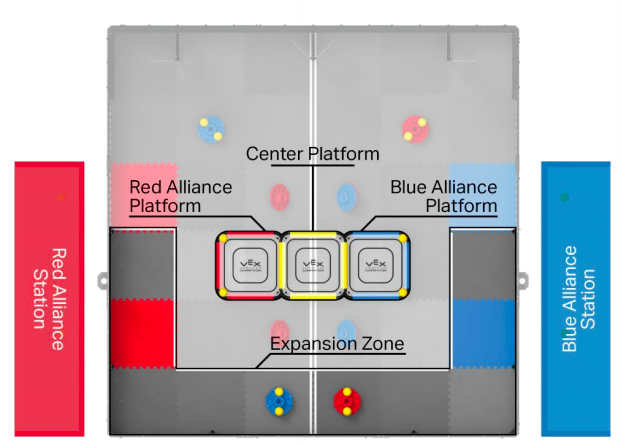
\includegraphics[width=.9\linewidth]{field/expansion}
    \caption{The Expansion Zone}
   \label{fig:expansionzone}
\end{figure}

\end{document}
